% Zeno's room: successive halves of a segment of length 1.
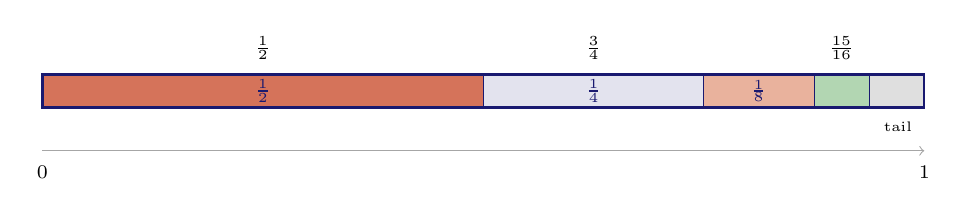
\begin{tikzpicture}[x=11.2cm,y=1cm]
  \fill[BrickRed!55] (0,0) rectangle (0.5,0.42);
  \fill[MidnightBlue!12] (0.5,0) rectangle (0.75,0.42);
  \fill[BrickRed!28] (0.75,0) rectangle (0.875,0.42);
  \fill[ForestGreen!35] (0.875,0) rectangle (0.9375,0.42);
  \fill[gray!25] (0.9375,0) rectangle (1,0.42);
  \draw[MidnightBlue,line width=0.8pt] (0,0) rectangle (1,0.42);
  \foreach \x in {0.5,0.75,0.875,0.9375} {
    \draw[MidnightBlue,line width=0.4pt] (\x,0) -- (\x,0.42);
  }
  \node[font=\scriptsize,MidnightBlue] at (0.25,0.21) {$\frac12$};
  \node[font=\scriptsize,MidnightBlue] at (0.625,0.21) {$\frac14$};
  \node[font=\tiny,MidnightBlue] at (0.812,0.21) {$\frac18$};
  \node[font=\scriptsize,anchor=south] at (0.25,0.48) {$\frac12$};
  \node[font=\scriptsize,anchor=south] at (0.625,0.48) {$\frac34$};
  \node[font=\scriptsize,anchor=south] at (0.906,0.48) {$\frac{15}{16}$};
  \node[font=\tiny,anchor=north] at (0.97,-0.06) {tail};
  \draw[gray!70,->] (0,-0.55) -- (1,-0.55);
  \node[font=\scriptsize,anchor=north] at (0,-0.62) {$0$};
  \node[font=\scriptsize,anchor=north] at (1,-0.62) {$1$};
\end{tikzpicture}
